% --- LaTeX Homework Template - S. Venkatraman ---

% --- Set document class and font size ---

\documentclass[letterpaper, 11pt]{article}

% --- Package imports ---

\usepackage{
  amsmath, amsthm, amssymb, mathtools, dsfont,	  % Math typesetting
  graphicx, wrapfig, subfig, float,                  % Figures and graphics formatting
  listings, color, inconsolata, pythonhighlight,     % Code formatting
  algorithm,algorithmic,fancyhdr, sectsty, hyperref, enumerate, enumitem } % Headers/footers, section fonts, links, lists

% --- Page layout settings ---

% Set page margins
\usepackage[left=1.35in, right=1.35in, bottom=1in, top=1.1in, headsep=0.2in]{geometry}

% Anchor footnotes to the bottom of the page
\usepackage[bottom]{footmisc}

% Set line spacing
\renewcommand{\baselinestretch}{1.2}

% Set spacing between paragraphs
\setlength{\parskip}{1.5mm}

% Allow multi-line equations to break onto the next page
\allowdisplaybreaks

% Enumerated lists: make numbers flush left, with parentheses around them
\setlist[enumerate]{wide=0pt, leftmargin=21pt, labelwidth=0pt, align=left}
\setenumerate[1]{label={(\arabic*)}}

% --- Page formatting settings ---

% Set link colors for labeled items (blue) and citations (red)
\hypersetup{colorlinks=true, linkcolor=blue, citecolor=red}

% Make reference section title font smaller
\renewcommand{\refname}{\large\bf{References}}

% --- Settings for printing computer code ---

% Define colors for green text (comments), grey text (line numbers),
% and green frame around code
\definecolor{greenText}{rgb}{0.5, 0.7, 0.5}
\definecolor{greyText}{rgb}{0.5, 0.5, 0.5}
\definecolor{codeFrame}{rgb}{0.5, 0.7, 0.5}

% Define code settings
\lstdefinestyle{code} {
  frame=single, rulecolor=\color{codeFrame},            % Include a green frame around the code
  numbers=left,                                         % Include line numbers
  numbersep=8pt,                                        % Add space between line numbers and frame
  numberstyle=\tiny\color{greyText},                    % Line number font size (tiny) and color (grey)
  commentstyle=\color{greenText},                       % Put comments in green text
  basicstyle=\linespread{1.1}\ttfamily\footnotesize,    % Set code line spacing
  keywordstyle=\ttfamily\footnotesize,                  % No special formatting for keywords
  showstringspaces=false,                               % No marks for spaces
  xleftmargin=1.95em,                                   % Align code frame with main text
  framexleftmargin=1.6em,                               % Extend frame left margin to include line numbers
  breaklines=true,                                      % Wrap long lines of code
  postbreak=\mbox{\textcolor{greenText}{$\hookrightarrow$}\space} % Mark wrapped lines with an arrow
}

% Set all code listings to be styled with the above settings
\lstset{style=code}

% --- Math/Statistics commands ---

% Add a reference number to a single line of a multi-line equation
% Usage: "\numberthis\label{labelNameHere}" in an align or gather environment
\newcommand\numberthis{\addtocounter{equation}{1}\tag{\theequation}}

% Shortcut for bold text in math mode, e.g. $\b{X}$
\let\b\mathbf

% Shortcut for bold Greek letters, e.g. $\bg{\beta}$
\let\bg\boldsymbol

% Shortcut for calligraphic script, e.g. %\mc{M}$
\let\mc\mathcal

% \mathscr{(letter here)} is sometimes used to denote vector spaces
\usepackage[mathscr]{euscript}

% Convergence: right arrow with optional text on top
% E.g. $\converge[w]$ for weak convergence
\newcommand{\converge}[1][]{\xrightarrow{#1}}

% Normal distribution: arguments are the mean and variance
% E.g. $\normal{\mu}{\sigma}$
\newcommand{\normal}[2]{\mathcal{N}\left(#1,#2\right)}

% Uniform distribution: arguments are the left and right endpoints
% E.g. $\unif{0}{1}$
\newcommand{\unif}[2]{\text{Uniform}(#1,#2)}

% Independent and identically distributed random variables
% E.g. $ X_1,...,X_n \iid \normal{0}{1}$
\newcommand{\iid}{\stackrel{\smash{\text{iid}}}{\sim}}

% Equality: equals sign with optional text on top
% E.g. $X \equals[d] Y$ for equality in distribution
\newcommand{\equals}[1][]{\stackrel{\smash{#1}}{=}}

% Math mode symbols for common sets and spaces. Example usage: $\R$
\newcommand{\R}{\mathbb{R}}   % Real numbers
\newcommand{\C}{\mathbb{C}}   % Complex numbers
\newcommand{\Q}{\mathbb{Q}}   % Rational numbers
\newcommand{\Z}{\mathbb{Z}}   % Integers
\newcommand{\N}{\mathbb{N}}   % Natural numbers
\newcommand{\F}{\mathcal{F}}  % Calligraphic F for a sigma algebra
\newcommand{\El}{\mathcal{L}} % Calligraphic L, e.g. for L^p spaces

% Math mode symbols for probability
\newcommand{\pr}{\mathbb{P}}    % Probability measure
\newcommand{\E}{\mathbb{E}}     % Expectation, e.g. $\E(X)$
\newcommand{\var}{\text{Var}}   % Variance, e.g. $\var(X)$
\newcommand{\cov}{\text{Cov}}   % Covariance, e.g. $\cov(X,Y)$
\newcommand{\corr}{\text{Corr}} % Correlation, e.g. $\corr(X,Y)$
\newcommand{\B}{\mathcal{B}}    % Borel sigma-algebra

% Other miscellaneous symbols
\newcommand{\tth}{\text{th}}	% Non-italicized 'th', e.g. $n^\tth$
\newcommand{\Oh}{\mathcal{O}}	% Big-O notation, e.g. $\O(n)$
\newcommand{\1}{\mathds{1}}	% Indicator function, e.g. $\1_A$

% Additional commands for math mode
\DeclareMathOperator*{\argmax}{argmax}    % Argmax, e.g. $\argmax_{x\in[0,1]} f(x)$
\DeclareMathOperator*{\argmin}{argmin}    % Argmin, e.g. $\argmin_{x\in[0,1]} f(x)$
\DeclareMathOperator*{\spann}{Span}       % Span, e.g. $\spann\{X_1,...,X_n\}$
\DeclareMathOperator*{\bias}{Bias}        % Bias, e.g. $\bias(\hat\theta)$
\DeclareMathOperator*{\ran}{ran}          % Range of an operator, e.g. $\ran(T) 
\DeclareMathOperator*{\dv}{d\!}           % Non-italicized 'with respect to', e.g. $\int f(x) \dv x$
\DeclareMathOperator*{\diag}{diag}        % Diagonal of a matrix, e.g. $\diag(M)$
\DeclareMathOperator*{\trace}{trace}      % Trace of a matrix, e.g. $\trace(M)$

% Numbered theorem, lemma, etc. settings - e.g., a definition, lemma, and theorem appearing in that 
% order in Section 2 will be numbered Definition 2.1, Lemma 2.2, Theorem 2.3. 
% Example usage: \begin{theorem}[Name of theorem] Theorem statement \end{theorem}
\theoremstyle{definition}
\newtheorem{theorem}{Theorem}[section]
\newtheorem{proposition}[theorem]{Proposition}
\newtheorem{lemma}[theorem]{Lemma}
\newtheorem{corollary}[theorem]{Corollary}
\newtheorem{definition}[theorem]{Definition}
\newtheorem{example}[theorem]{Example}
\newtheorem{remark}[theorem]{Remark}

% Un-numbered theorem, lemma, etc. settings
% Example usage: \begin{lemma*}[Name of lemma] Lemma statement \end{lemma*}
\newtheorem*{theorem*}{Theorem}
\newtheorem*{proposition*}{Proposition}
\newtheorem*{lemma*}{Lemma}
\newtheorem*{corollary*}{Corollary}
\newtheorem*{definition*}{Definition}
\newtheorem*{example*}{Example}
\newtheorem*{remark*}{Remark}
\newtheorem*{claim}{Claim}

% --- Left/right header text (to appear on every page) ---

% Include a line underneath the header, no footer line
\pagestyle{fancy}
\renewcommand{\footrulewidth}{0pt}
\renewcommand{\headrulewidth}{0.4pt}
\newcommand{\homework}[1]{
   \pagestyle{myheadings}
   \thispagestyle{plain}
   \newpage
   \setcounter{page}{1}
   \noindent
   \classname \hfill \mbox{\updatedday} \\
   \instname \hfill \mbox{\duedate}
   \rule{6.5in}{0.5mm}
   \vspace*{-0.1 in}
}


\newcommand{\problem}[1]{\section*{Problem #1}}


\renewcommand{\labelenumi}{(\alph{enumi})}
\renewcommand{\labelenumii}{(\roman{enumii})}
\newenvironment{solution}{{\par\noindent\it Solution.}}{}
% Left header text: course name/assignment number
\lhead{CSCI-SHU 220: Algorithms\\Homework 1}

% Right header text: your name
\rhead{Posted: February 11, 2025\\Due: 11:55pm (Shanghai time), February 25, 2025}

% --- Document starts here ---

\begin{document}

This assignment has a total of $90$ base points and $10$ extra points, and the cap is $90$.
%Typesetting your solution using \LaTeX\ (by simply editing this tex template) gains $5$ extra points.
Bonus questions are indicated using the $\star$ mark.

Submission Instructions: Please submit to Gradescope (we will post the link later in the announcements). During submission, you need to \textbf{mark/map the solution to each question}; otherwise, we may apply a penalty. 

Another notice: you only get full credits for the algorithm design questions if your algorithm matches the desirable complexity. If the desirable complexity is not stated, you need to design an algorithm to be as fast as possible.

\textit{Please specify the following information before submission}:
\begin{itemize}
    \item Your Name: Yixia Yu
    \item Your NetID: yy5091
\end{itemize}


\problem{1: Asymptotic analysis [$5 \times 4$ pts]} 
\begin{enumerate}
    \item What's the asymptotic relationship between $f(n) = (\log\log n)^{\log n}$ and $g(n) = \log^{\log\log n}n$ and prove it?
    \item What's the asymptotic relationship between $f(n) = 1 + \frac{1}{2} + \frac{1}{3} + \ldots \frac{1}{n}$ and $g(n) = \sum_{i=1}^{n} 2^{-\lceil\log i \rceil}$ and prove it?
    \item Prove that $n! = \omega(n^{0.99n})$.
    
    \item In the practice table from the lecture, we have examples of $f$ and $g$ satisfying the following combinations of asymptotic relationships: $\{O, o\}$, $\{\Omega, \omega\}$, and $\{\Theta, O, \Omega\}$. Are there any other possible combinations? For every combination not in the listed three (combination also includes the empty set, or any singleton), construct an example of $f$ and $g$ and prove it.
    
    \item What's the asymptotic relationship between $f(n)=n^{0.6}$ and $g(n) = 2^{2^{\lfloor \log\log n \rfloor}}$ and prove it?
    
    \end{enumerate}
    \begin{solution}
        (1)
    \begin{align*}
        f(n) &= \omega  g(n) \\
    \end{align*}
    Proof:
        \begin{align*}
        \log{f(n)} &= \log{(\log\log n)^{\log n}} \\
        &= \log n{\log (\log\log n)} \\
        \log{g(n)} &= \log{(\log^{\log\log n}n)} \\
        &= \log \log n\log ( \log n) \\
        \text{Since }\frac{\log n}{(\log ( \log n))^2} &\rightarrow +\infty \text{ as } n\rightarrow +\infty \\
        \lim_{n\rightarrow +\infty}\frac{f(n)}{g(n)}&= \frac{\log n{\log (\log\log n)}}{(\log ( \log n))^2}=+\infty  \\
        \text{So, }f(n) &= \omega  g(n) \\
    \end{align*}
    (2): \begin{align*}{}{}
    \text{Since }\log i \leq \lceil\log i \rceil &\leq \log i + 1 \\
    \text{Then, } 2^{-\lceil\log i \rceil}&\geq 2^{-\log i - 1}=\frac{1}{2i}\\
    \text{And }2^{-\lceil\log i \rceil}&\leq 2^{-\log i}=\frac{1}{i}\\
    \text{So, } \frac{1}{2}\sum_{i=1}^{n} \frac{1}{i}\leq&\sum_{i=1}^{n} 2^{-\lceil\log i \rceil}\leq\sum_{i=1}^{n} \frac{1}{i} \\
    \text{Thus, } 1 + \frac{1}{2} + \frac{1}{3} + \ldots \frac{1}{n}&=\Theta \sum_{i=1}^{n} 2^{-\lceil\log i \rceil} \\
    \text{i.e. } f(n)&=\Theta g(n) \\
   \end{align*} 
   (3):\begin{align*}
    \text{We first prove that } \log n! &= \Theta(n\log n)\\
    \text{Since } log(n!)&=log(1)+log(2)+\ldots+log(n)\\
    \text{We have by monotonicity: }log(n!)&\leq \sum_{k=1}^{n}log(n)=nlog(n)\\
    \text{From the bound, we can}&\text{ use the fact that }log(k)\geq log(\frac{n}{2}), \forall k\geq2\\
    \text{Thus, we can }\text{get:}&\\
    log(n!)\geq \sum_{k=\frac{n}{2}}^{n}log(k)&\geq \sum_{k=\frac{n}{2}}^{n}log(\frac{n}{2})=\frac{n}{2}log(\frac{n}{2})\\
    \text{Since } \log n! &= \Theta(n\log n) \\
    \text{And } \log(n^{0.99n}) &=0.99n\log n= o(n\log n) \\
    \text{So, } n! &= \omega(n^{0.99n}) \\
    \end{align*}
    (4): \begin{align*}
    \text{The possible combinations are: }\emptyset,\{\Omega\},\{O\}\\
    \text{For }\emptyset, \text{we can have: }f(n)&=n, g(n) = n^{1+\sin(n)}\\
    \text{For }\{\Omega\}, \text{we can have: }f(n)&=\begin{cases}
        n^2, & \text{if } n \text{ is even} \\
        n, & \text{if } n \text{ is odd}
    \end{cases}, g(n)=n\\
    \text{For }\{O\}, \text{we can have: }f(n)&= n \sin^2(n), g(n)=n\\
    \end{align*}
    (5): 
    The asymptotic relationship is empty set $ \emptyset $ \\
    Since we have\begin{align*}
        2^{2^{\log\log n -1}}\leq 2^{2^{\lfloor \log\log n \rfloor}}\leq 2^{2^{ \log\log n }}\\
        2^{0.5\log n}\leq 2^{2^{\lfloor \log\log n \rfloor}}\leq2^{\log n}\\
        n^{0.5}\leq 2^{2^{\lfloor \log\log n \rfloor}}\leq n
        \end{align*}
    Since $ n^{0.5}\leq n^{0.6}\leq n $ ,then $$
        \liminf_{n\rightarrow +\infty}\frac{f(n)}{g(n)}=0, \limsup_{n\rightarrow +\infty}\frac{f(n)}{g(n)}=+\infty
    $$ 
    So, $f(n)=\emptyset g(n)$
\end{solution}
\problem{2: Finding the maximum/minimum [$10+10^\star$ pts]}
For an array $A$ of $n$ \textit{different} numbers (not necessarily sorted), we want to find the \textit{largest} number and the \textit{smallest} number in $A$ simultaneously.
However, we have no access to $A$.
Instead, we are given an oracle $\textsc{Compare}$ that can be used to compare the numbers in $A$.
For $i \neq j$, $\textsc{Compare}(i,j)$ returns $i$ if $A[i]>A[j]$ and returns $j$ if $A[j]>A[i]$ (recall that the numbers in $A$ are different by assumption, so we cannot have $A[i]=A[j]$ if $i \neq j$).
For convenience, let us assume $n$ is even.
\begin{enumerate}
    \item Design an algorithm which calls the $\textsc{Compare}$ oracle at most $\frac{3}{2} n - 2$ times and returns a pair $(i_\mathsf{max},i_\mathsf{min})$ such that $A[i_\mathsf{max}]$ (resp., $A[i_\mathsf{min}]$) is the largest (resp., smallest) number in $A$. Give the pseudocode and justify its correctness.
    %
    %(\textbf{Hint:} Divide the numbers in $A$ into $n/2$ groups of size 2, compare the two numbers in each group, and then based on the outcome try to find $i_\mathsf{max},i_\mathsf{min}$ with $n-2$ additional comparisons.)
    
    \item[(b)$^\star$] Show that any algorithm has to call the $\textsc{Compare}$ oracle $\frac{3}{2} n - 2$ times in worst case in order to find the largest and smallest numbers in $A$.

\end{enumerate}

\begin{solution}
    \begin{algorithm}[H]
        \begin{algorithmic}[1]
            \STATE Initialize empty lists: \texttt{CandidatesMax} and \texttt{CandidatesMin}
            \FOR{$i=1$ to $n-1$ step 2}
                \IF{\textsc{Compare}$(i, i+1)$ = $i$}
                    \STATE Append $i$ to \texttt{CandidatesMax}
                    \STATE Append $i+1$ to \texttt{CandidatesMin}
                \ELSE
                    \STATE Append $i+1$ to \texttt{CandidatesMax}
                    \STATE Append $i$ to \texttt{CandidatesMin}
                \ENDIF
            \ENDFOR
            \STATE $i_\mathsf{max} \gets$ \texttt{CandidatesMax}[0]
            \FOR{each index $j$ in \texttt{CandidatesMax}}
                \IF{\textsc{Compare}$(j, i_\mathsf{max})$ = $j$}
                    \STATE $i_\mathsf{max} \gets j$
                \ENDIF
            \ENDFOR
            \STATE $i_\mathsf{min} \gets$ \texttt{CandidatesMin}[0]
            \FOR{each index $j$ in \texttt{CandidatesMin}}
                \IF{\textsc{Compare}$(j, i_\mathsf{min})$ = $i_\mathsf{min}$}
                    \STATE $i_\mathsf{min} \gets j$
                \ENDIF
            \ENDFOR
            \ENSURE $(i_\mathsf{max}, i_\mathsf{min})$
        \end{algorithmic}
        \caption{Find the maximum and minimum indices in array $A$ using at most $\frac{3n}{2} - 2$ comparisons}
        \end{algorithm}
        \textbf{Correctness:}
        \\The core idea is to reduce the number of candidates for both maximum and minimum in a single pass. By comparing elements pairwise, we guarantee that for each comparison, one element goes to the potential maximum list and the other to the potential minimum list. This effectively halves the number of elements we need to consider in subsequent steps. The separate loops for finding the maximum and minimum among the candidates then efficiently determine the true maximum and minimum indices. The algorithm's correctness stems from the transitivity of the comparison: if a > b and b > c, then a > c. The pairwise comparisons, combined with the subsequent candidate refinement, ensure that the true maximum and minimum are identified.
      \\ (b) \begin{proof}
            Let us define two sets:
\begin{itemize}
    \item $MAX$: set of elements that could still be the maximum
    \item $MIN$: set of elements that could still be the minimum
\end{itemize}

Initially, all $n$ elements belong to both $MAX$ and $MIN$. To determine the maximum and minimum, the algorithm must eliminate $n-1$ elements from $MAX$ and $n-1$ elements from $MIN$, for a total of $2n-2$ eliminations.

The crucial insight is that a single comparison can eliminate at most 2 elements, one from each set. Specifically:
\begin{itemize}
    \item When $\textsc{Compare}(i,j)$ returns $i$, we can eliminate $j$ from $MAX$ and $i$ from $MIN$.
    \item When $\textsc{Compare}(i,j)$ returns $j$, we can eliminate $i$ from $MAX$ and $j$ from $MIN$.
\end{itemize}

However, this maximum efficiency (eliminating 2 elements per comparison) is only possible when both elements being compared are in $MAX \cap MIN$. Once an element has been eliminated from one set but remains in the other, comparing it can only eliminate at most one element.

The optimal strategy involves first pairing up the elements and comparing each pair. After $\frac{n}{2}$ such comparisons:
\begin{itemize}
    \item $\frac{n}{2}$ elements (the winners) remain in $MAX$ but are eliminated from $MIN$
    \item $\frac{n}{2}$ elements (the losers) remain in $MIN$ but are eliminated from $MAX$
\end{itemize}

At this point, we've eliminated $\frac{n}{2}$ elements from each set, with $\frac{n}{2}$ elements remaining in each. To determine the maximum, we need to eliminate $\frac{n}{2}-1$ more elements from $MAX$, requiring at least $\frac{n}{2}-1$ additional comparisons. Similarly, determining the minimum requires eliminating $\frac{n}{2}-1$ more elements from $MIN$, needing at least $\frac{n}{2}-1$ more comparisons.

Therefore, the total number of comparisons is at least:
$$\frac{n}{2} + \left(\frac{n}{2}-1\right) + \left(\frac{n}{2}-1\right) = \frac{3n}{2} - 2$$
                \end{proof}
\end{solution}

\problem{3: Solving recurrences [$4 \times 5+5$ pts]}
\begin{enumerate}
    \item Find big-$\Theta$ bounds for the following recurrences (and show your bounds are correct). For the base case, simply assume $T(n) = 1$ for all $n \leq 2$.
    \begin{enumerate}
        \item $T(n)=8T(n/3)+n^{1.5} \log^4 n + 9n$
        \item $T(n)=T(n-\sqrt{n}) + 6 \log n$
        \item $T(n)=2T(n/2)+ \frac{n}{\log n}$
        \item $T(n)= 5\sqrt{n} \cdot T(\sqrt{n}) + 2n$
    \end{enumerate}
    \item Recall the Fibonacci sequence $F_0,F_1,F_2,\dots$ defined using the recurrence $F_n = F_{n-1}+F_{n-2}$ with the base case $F_0 = 0$ and $F_1 = 1$. Prove by induction that $\phi^{n-2} \leq F_n < \phi^n$ for all $n \geq 1$, where $\phi = (1+\sqrt{5})/2$.
    Based on this, further show that $F_n = \Theta(\phi^n)$.
\end{enumerate}

\begin{solution}
    \begin{enumerate}
        \item
       \begin{enumerate}
            \item  By master theorem, we have $a=8, b=3, f(n)=n^{1.5} \log^4 n + 9n$. Since $f(n)=O(n^{\log_3 8-\epsilon})$ for $\epsilon=0.5$, we have $T(n)=\Theta(n^{\log_3 8})$.
            \item Let $m=\sqrt{n}$, then we have $T(m^2)=T(m^2-m)+12\log m$. \\
            So we have $ T((m^2)=T(m-0.5)^2)+12\log m -0.25 $ \\
            Let $S(m)=T(m^2)$\\
            So we have $S(m)=S(m-0.5)+12\log m -0.25$\\
            Since the step is 0.5, we have $S(m)=\Theta(m\log m)$\\
            So we have $T(n)=\Theta(\sqrt{n}\log \sqrt{n})=\Theta(\sqrt{n}\log n)$
            \item By recursion tree, the i-th layer has the sum $ \frac{n}{\log \frac{n}{i}} $ and we have $\log n -1 $ layers 
            \\So we have $T(n) = \sum_{i=0}^{\log n-1} \frac{n}{\log n - i}$

            Let $j = \log n - i$. We have
            \begin{align*}
            T(n) &= \sum_{i=0}^{\log n-1} \frac{n}{\log n - i} \\
            &= \sum_{j=\log n}^{1} \frac{n}{j} \cdot (-1)  \\
            &= n \sum_{j=1}^{\log n} \frac{1}{j} 
            \end{align*}
            
  we observe that:
            
            \begin{align*}
            \int_{1}^{\log n} \frac{1}{x}\,dx < \sum_{j=1}^{\log n} \frac{1}{j} < 1 + \int_{1}^{\log n} \frac{1}{x}\,dx
            \end{align*}
            
            This gives us:
            \begin{align*}
            \ln(\log n) < \sum_{j=1}^{\log n} \frac{1}{j} < 1 + \ln(\log n)
            \end{align*}
            
            In fact, it can be shown that as $n$ grows large:
            \begin{align*}
            \sum_{j=1}^{\log n} \frac{1}{j} = \ln(\log n) + \gamma + O\left(\frac{1}{\log n}\right)
            \end{align*}
            
            where $\gamma \approx 0.57721$ is the Euler-Mascheroni constant.
            
            Therefore, the original sum has the asymptotic behavior:
            \begin{align*}
            T(n) &= n \sum_{j=1}^{\log n} \frac{1}{j} \\
            &= n \cdot (\ln(\log n) + \gamma + o(1)) \\
            &= n\ln(\log n) + \gamma n + o(n) \\
            &= \Theta(n\log\log n)
            \end{align*}
            
            Thus, $T(n) = \Theta(n\log\log n)$.
            \item Let $ n=2^m,S(m)=T(2^m)=T(n) $, then we have
            $$
                S(m)=5\cdot 2^{m/2}\cdot S(m/2)+2^{m+1}
            $$ 
            Divide both sides by $2^{m}$, we have
            \begin{align*}{}{}
            \frac{S(m)}{2^{m}}&=5\cdot \frac{S(m/2)}{2^{-m/2}}+2\\
            \text{Let }P(m)&=\frac{S(m)}{2^{m}}\\
            P(m)&=5\cdot P(m/2)+2\\
            \text{By master theorem, we have }a&=5, b=2, f(m)=2\\
            \text{Since }f(m)&=O(m^{\log_2 5-\epsilon}) \text{ for } \epsilon=1\\
            \text{we have }P(m)&=\Theta(m^{\log_2 5})\\
            \text{So, }S(m)&=\Theta(2^m\cdot m^{\log_2 5})\\
            \text{Thus, }T(n)&=\Theta(n\cdot (\log n)^{\log_2 5})\\
            \end{align*}
        \end{enumerate}
        \item When $n=1$, we have $F_n=1$ and $\phi^{n-2}=\frac{2}{1+\sqrt{5}}$.\\
        So we have $\phi^{n-2} \leq F_n < \phi^n$ for $n=1$.\\
        Assume that $\phi^{n-2} \leq F_n < \phi^n$ for $n=k$, \\
        then we have $F_{k+1}=F_k+F_{k-1}<\phi^k+\phi^{k-1}=\phi^{k-1}(\phi+1)=\phi^{k-1}\phi^2=\phi^{k+1}$\\
        And $F_{k+1}=F_k+F_{k-1}>\phi^{k-2}+\phi^{k-1}=\phi^{k-2}(\phi+1)=\phi^{k-2}\phi^2=\phi^{k}$
        So we have $\phi^{n-2} \leq F_n < \phi^n$ for all $n \geq 1$\\
        Since $\phi^{n}\cdot \underbrace{\phi^{-2}}_{constant} \leq F_n < \phi^n$ for all $n \geq 1$, we have $F_n = \Theta(\phi^n)$
    \end{enumerate}
\end{solution}
\problem{4: Counting intersection points [$10$ pts]}
Consider two horizontal lines $\ell_0: y = 0$ and $\ell_1:y = 1$ in the plane.
We have $n$ distinct points $a_1,\dots,a_n$ on $\ell_0$ and $n$ distinct points $b_1,\dots,b_n$ on $\ell_1$.
Note that the points $a_1,\dots,a_n$ and $b_1,\dots,b_n$ are \textit{not} necessarily sorted by their $x$-coordinates.
Now for each $i \in \{1,\dots,n\}$, we draw a segment $s_i$ connecting $a_i$ and $b_i$.
See the figure below for an example of $n = 4$.
These segments $s_1,\dots,s_n$ may intersect with each other, and for simplicity, we assume no three segments intersect at the same point.
We aim to count the number of intersection points of $s_1,\dots,s_n$.

Formally, design an algorithm $\textsc{CountInt}(n,A,B)$ where $A[1 \dots n]$ stores the $x$-coordinates of $a_1,\dots,a_n$ and $B[1 \dots n]$ stores the $x$-coordinates of $b_1,\dots,b_n$.
The algorithm should return the number of intersection points of the segments $s_1,\dots,s_n$, and should have time complexity $O(n \log n)$.
Describe the basic idea and give the pseudocode.
Then, justify its correctness and show it runs in $O(n \log n)$ time.

\begin{center}
    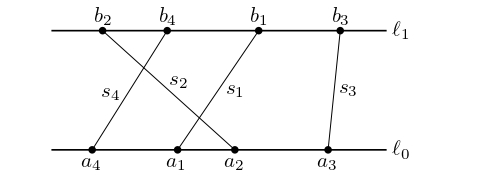
\includegraphics[height=4cm]{hw-fig-intersection.jpg}
\end{center}

\begin{solution}
Observing that for every points on $ l_1 \text{ and } l_0 $ , we will have one intersection point when comparing k-th points (from left to right) on $ l_1 \text{ and } l_0 $ and have i>j for $ a_i \text{ and } b_j $ because under this condition, $b_i>b_j \text{ and } a_i<a_j   $ 
\\So the idea is to merge sort on $ a_1,a_2,\cdots,a_n $ and $ b_1,b_2,\cdots,b_n $ to get the sorted position from them, then compare each index with corresponding postion's index of $ b_1,b_2,\cdots,b_n $ to get the number of intersection points.
\begin{algorithm}[H]
    \caption{Count Intersection Points}
    \begin{algorithmic}[1]
    \STATE \textbf{Function} \textsc{CountInt}$(n, A, B)$
    \STATE Create pairs $P_A[1...n]$ where $P_A[i] = (A[i], i)$ for $i = 1$ to $n$
    \STATE Create pairs $P_B[1...n]$ where $P_B[i] = (B[i], i)$ for $i = 1$ to $n$
    \STATE \textsc{MergeSort}$(P_A, 1, n)$ \COMMENT{Sort by first element}
    \STATE \textsc{MergeSort}$(P_B, 1, n)$ \COMMENT{Sort by first element}
    \STATE Create arrays $I[1...n]$ and $J[1...n]$
    \FOR{$i = 1$ to $n$}
    \STATE $I[i] \gets $ second element of $P_A[i]$
    \STATE $J[i] \gets $ second element of $P_B[i]$
    \ENDFOR
    \STATE $count \gets 0$
    \FOR{$i = 1$ to $n$}
    \IF{$J[i] > I[i]$}
    \STATE $count \gets count + 1$
    \ENDIF
    \ENDFOR
    \RETURN $count$
    \end{algorithmic}
    \end{algorithm}
    
    \begin{algorithm}[H]
    \caption{Merge Sort}
    \begin{algorithmic}[1]
    \STATE \textbf{Function} \textsc{MergeSort}$(P, left, right)$
    \IF{$left < right$}
    \STATE $mid \gets \lfloor(left + right)/2\rfloor$
    \STATE \textsc{MergeSort}$(P, left, mid)$
    \STATE \textsc{MergeSort}$(P, mid+1, right)$
    \STATE \textsc{Merge}$(P, left, mid, right)$
    \ENDIF
    \end{algorithmic}
    \end{algorithm}
    
    \begin{algorithm}[H]
    \caption{Merge}
    \begin{algorithmic}[1]
    \STATE \textbf{Function} \textsc{Merge}$(P, left, mid, right)$
    \STATE Create temporary arrays $L[1...(mid-left+1)]$ and $R[1...(right-mid)]$
    \STATE Copy $P[left...mid]$ to $L$ and $P[mid+1...right]$ to $R$
    \STATE $i \gets 1, j \gets 1, k \gets left$
    \WHILE{$i \leq (mid-left+1)$ AND $j \leq (right-mid)$}
    \IF{$L[i].first \leq R[j].first$}
    \STATE $P[k] \gets L[i]$
    \STATE $i \gets i + 1$
    \ELSE
    \STATE $P[k] \gets R[j]$
    \STATE $j \gets j + 1$
    \ENDIF
    \STATE $k \gets k + 1$
    \ENDWHILE
    \WHILE{$i \leq (mid-left+1)$}
    \STATE $P[k] \gets L[i]$
    \STATE $i \gets i + 1$
    \STATE $k \gets k + 1$
    \ENDWHILE
    \WHILE{$j \leq (right-mid)$}
    \STATE $P[k] \gets R[j]$
    \STATE $j \gets j + 1$
    \STATE $k \gets k + 1$
    \ENDWHILE
    \end{algorithmic}
    \end{algorithm}
\textbf{Correctness:} The algorithm sorts the points on $l_0$ and $l_1$ by their $x$-coordinates. For every points on $ l_1 \text{ and } l_0 $ , we will have one intersection point when comparing k-th points (from left to right) on $ l_1 \text{ and } l_0 $ and have i>j for $ a_i \text{ and } b_j $ because under this condition, $b_i>b_j \text{ and } a_i<a_j   $ 
\\\textbf{Complexity:} The algorithm sorts the points on $l_0$ and $l_1$ by their $x$-coordinates in $O(n\log n)$ time. Then, it compares the indices of the sorted points in $O(n)$ time. Thus, the total time complexity is $O(n\log n)$.
\end{solution}


\problem{5: 3SUM from 3 arrays [$8$ pts]}
Given 3 non-empty and sorted arrays $A, B, C$ of integers, each array is of size $N_A$, $N_B$ and $N_C$ respectively. Given an input $a$, output one value from each array such that the sum is equal to $a$. If not found, return $0$. Design the algorithm, prove its correctness and complexity.

\begin{solution}
    \begin{algorithm}[H]
        \caption{3SUM from 3 arrays}
        \begin{algorithmic}[1]
        \STATE \textbf{Function} {FindTriplet}{$A, B, C, a$}
            \STATE  $NA \gets \text{length}(A)$
            \STATE  $NB \gets \text{length}(B)$
            \STATE  $NC \gets \text{length}(C)$
            \FOR{$i = 1$ to $NA$}
                \STATE  $target \gets a - A[i]$
                \STATE $j \gets 1$
                \STATE  $k \gets NC$
                \WHILE{$j \leq NB$ \textbf{and} $k \geq 1$}
                    \STATE $s \gets B[j] + C[k]$
                    \IF{$s = target$}
                    \RETURN $(A[i], B[j], C[k])$
                    \ELSIF{$s < target$}
                        \STATE  $j \gets j + 1$
                    \ELSE
                        \STATE $k \gets k - 1$
                    \ENDIF
                \ENDWHILE
            \ENDFOR
            \RETURN $0$
        \end{algorithmic}
        \end{algorithm}
    \textbf{Correctness:}\\ 
    The algorithm is correct because it systematically fixes each candidate from array A and uses a correctly implemented two-pointer method on two sorted arrays B and C to find complementary pairs that sum to the required value. This ensures that, if a valid triplet exists, it will be found.     
\\\textbf{Complexity:}\\
The algorithm iterates through the elements of array A, and for each element, it uses a two-pointer method to find a pair in arrays B and C that sum to the target value. The two-pointer method takes $O(N_B + N_C)$ time, and since the algorithm iterates through all elements of array A, the total time complexity is $O(N_A(N_B + N_C))$.
\end{solution}    
\problem{6: Counting context-free grammar words [$7$ pts]}
Context-free grammar (CFG) is an important concept in CS, and it recursively defines a set of strings/words. You may want to search for CFG and learn about the relevant context. In this problem, we omit many formal definitions and focus on the following grammar:

\begin{enumerate}
    \item $S \rightarrow D | D + S$
    \item $D \rightarrow 1D | 2D | 3D | 4D | \ldots |9D |0|1|2|3|\ldots|9$
\end{enumerate}

The above two rules read as follows: we always start with $S$, and $S$ can either get turned into $D$ or $D+S$. Here, $+$ is a terminal symbol and cannot be transformed into other symbols. For the second rule, $D$ can get transformed into $1D$ or $2D$ or $\ldots$, and all the numbers are terminal symbols. The ``$|$'' essentially means ``or'' for the transformation. A word satisfying the above CFG is a string of terminal symbols that can be generated using the above rules.

Think about what the above grammar represents. Count the number of words satisfying the above CFG of a given length $n$ using recursion.


\begin{solution}
        \begin{algorithm}[H]
        \caption{f(n):Counting context-free grammar words }
        \begin{algorithmic}[1]
            \STATE \textbf{Function:} g(n)
            \IF{\(n = 1\)}
                \RETURN 10 
            \ELSE
                \RETURN \(9 \times g(n-1)\) 
            \ENDIF
        \STATE \textbf{Function:} f(n)
            \IF{\(n = 1\)}
                \RETURN g(1) 
            \ENDIF
            \STATE result \(\gets\) g(n) \COMMENT{Case 1: \(S \rightarrow D\).}
            \FOR{\(i \gets 1\) \TO \(n-2\)}
                \STATE result \(\gets\) result + g(i) \(\times\) f(n-i-1) \COMMENT{Case 2: \(S \rightarrow D + S\) }
            \ENDFOR
            \RETURN result
        \end{algorithmic}
        \end{algorithm}
\end{solution}

\problem{7: Search for a root [$10$ pts]}
Given a continuous function $f : [1,2]\times[1,2] \rightarrow [0,1]$ with the ``bi-monotone'' property: $f(x,y) > f(x',y)$ if $x > x'$ and $f(x,y) > f(x,y')$ if $y > y'$, we want to solve for the root of $f(x,y) = a$ where $a$ is some given value. The only access to $f$ is an oracle such that given $(x,y)$, the oracle returns the value of $f(x,y)$.

Let $R$ be the set of roots, i.e., $f(x^*,y^*) = a$ for any $(x^*,y^*) \in R$. We want to find an approximate solution $(\hat{x},\hat{y})$ such that there exists $(x^*,y^*) \in R$ with $\hat{x} \leq x^* \leq (1+\epsilon) \hat{x}$ and $\hat{y} \leq y^* \leq (1+\epsilon) \hat{y}$ with as few oracle calls as possible. Here, $\epsilon > 0$ is another given parameter indicating the desirable level of accuracy. If there is no root, return $0$.

Design an algorithm $\textsc{FindRoot}(f, a, \epsilon)$, and prove its correctness and complexity (in terms of number of oracle calls). \emph{This problem is a little bit more involved, but it does not require anything beyond the lectures. Suggest working on this after you finish everything else.}

\begin{solution}
    \begin{algorithm}[H]
        \caption{FindRoot: Approximate a solution $(x,y)$ for $f(x,y)=a$}
        \begin{algorithmic}[1]
            \STATE \textbf{Function:} FindRoot(f, a, $\epsilon$)
            \IF{\(f(1,1) > a \text{ or } f(2,2) < a\)}
                \RETURN 0 \COMMENT{No solution exists in $[1,2]\times[1,2]$}
            \ENDIF
            \STATE \(x_{\text{low}} \gets 1,\; x_{\text{high}}  \gets 2\)
            \WHILE{\(x_{\text{high}}  / x_{\text{low}}  > 1+\epsilon\)}
                \STATE \(x_{\text{mid}}  \gets \sqrt{x_{\text{low}}  \times x_{\text{high}} }\)
                \IF{\(a < f(x_{\text{mid}}  ,1)\)}
                    \STATE \(x_{\text{high}} \gets x_{\text{mid}}  \)
                \ELSIF{\(a > f(x_{\text{mid}}  ,2)\)}
                    \STATE \(x_{\text{low}}  \gets x_{\text{mid}}  \)
                \ELSE
                    \STATE \(x_{\text{high}}  \gets x_{\text{mid}}  \)
                \ENDIF
            \ENDWHILE
            \STATE \(\hat{x} \gets x_{\text{low}} \)
            \STATE \(y_{\text{low}} \gets 1,\; y_{\text{high}} \gets 2\)
            \WHILE{\(y_{\text{high}} / y_{\text{low}}> 1+\epsilon\)}
                \STATE \(y_{\text{mid}} \gets \sqrt{y_{\text{low}} \times y_{\text{high}} }\)
                \IF{\(f(\hat{x}, y_{\text{mid}} ) < a\)}
                    \STATE \(y_{\text{low}}\gets y_{\text{mid}} \)
                \ELSE
                    \STATE \(y_{\text{high}}  \gets y_{\text{mid}} \)
                \ENDIF
            \ENDWHILE
            \STATE \(\hat{y} \gets y_{\text{low}}\)
            \RETURN \((\hat{x}, \hat{y})\)
        \end{algorithmic}
        \end{algorithm}
        \textbf{Correctness:} \\
The algorithm is correct because it uses the strict monotonicity of \( f(x,y) \) in both variables to maintain intervals that always contain a true root. By performing a multiplicative binary search, the algorithm narrows the intervals until the relative error for both the \( x \) and \( y \) coordinates is at most \( 1+\epsilon \). This guarantees that there exists a true solution \( (x^*, y^*) \) with
\[
X_{\text{approx}} \le x^* \le (1+\epsilon)X_{\text{approx}} \quad \text{and} \quad
Y_{\text{approx}} \le y^* \le (1+\epsilon)Y_{\text{approx}},
\]
meeting the required approximation condition.

\textbf{Complexity:} \\
Each binary search (for both \( x \) and \( y \)) reduces the interval multiplicatively, starting from \([1,2]\) (a factor of 2) and ending when the interval ratio is at most \( 1+\epsilon \). This requires 
\(
O\bigl(\log_{1+\epsilon}(2)\bigr)
\)
iterations, which is approximately \( O(1/\epsilon) \) for small \( \epsilon \). Since each iteration makes a constant number of oracle calls, the total number of oracle calls is \( O(1/\epsilon) \).
\end{solution}


\end{document}
